\documentclass{beamer}
\usetheme{Antibes}
\usecolortheme{beaver}
\usepackage{graphicx}
\usepackage[slovak]{babel}
	
%-------------------
\author{Ondrej Krajčovič}
\institute{
    Ústav informatiky, informačných systémov a softvérového inžinierstva\\
    Fakulta informatiky a informačných technológií\\
    Slovenská technická univerzita v Bratislave
}
\subtitle{\vspace{3mm} Metódy inžinierskej práce 2023/2024}
\title{text-to-image search/ image-to-image search}
\date{\footnotesize 26. november 2023}
%-------------------
\begin{document}

\frame{\titlepage}

\begin{frame}
 \frametitle{Sémantika}
 \begin{itemize}
    \item Kde je možné stretnúť sa s text-to-image a image-to-image vyhľadávaním?
    \item Predstavte si nasledujúcu situáciu
\end{itemize}
\end{frame}

\begin{frame}
\frametitle{Metadata}
\begin{itemize}
    \item Čo sú metadáta?
    \item K čomu sa využívajú?
    	\begin{itemize}
	\item K čomu ich vieme využiť v text-to-image vyhľadávaní?
	\end{itemize}
\end{itemize}
\end{frame}

\begin{frame}
  \frametitle{Metadáta}
  \begin{figure}
    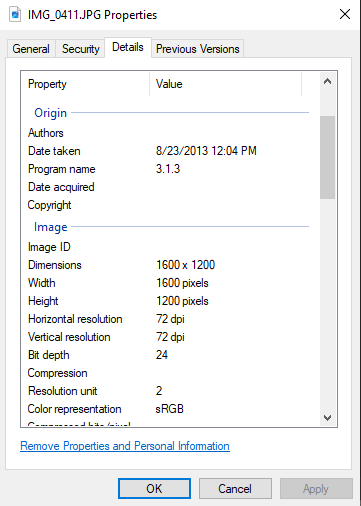
\includegraphics[width=0.4\textwidth]{metadata.png}[~\ref{metadata}]
    \caption{Príklad zobrazenia Metadát obrázku v prostredí windows}
  \end{figure}
\end{frame}

\begin{frame}
  \frametitle{Image-to-image search}
   \begin{itemize}
     \item Analýza vizuálnych prvkov(čŕt) obrázku na vstupe
     \item porovnávanie čŕt s inými obrázkami
     \item vyhľadanie najpodobnejších obrázkov
   \end{itemize}
\end{frame}

\begin{frame}
  \frametitle{Image-to-image search vs. text-to-image search}\label{diagram_slide}
  \begin{figure}
    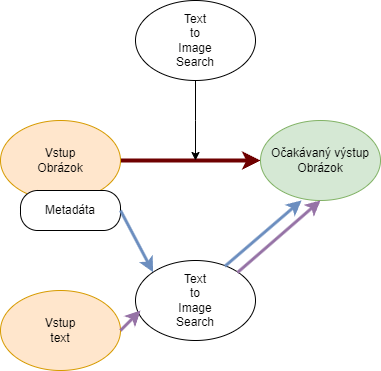
\includegraphics[width=0.5\textwidth]{Diagram_MIP_prez.png}[~\ref{diagram}]
    \caption{Diagram znázorňujúci procesy použité prí image-to-image a text-to-image vyhľadávaní}
  \end{figure}
\end{frame}

\begin{frame}
  \frametitle{AI}
     \begin{itemize}
     \item AI vie výrazne zefektívniť proces vyhľadávania
     \item Extrakcia textových dát opisujúcich obrázok, a následný text-to-image search [~\ref{diagram_slide}]
   \end{itemize}
\end{frame}

\begin{frame}
  \frametitle{CLIP Image from OpenAI}
  \begin{figure}
    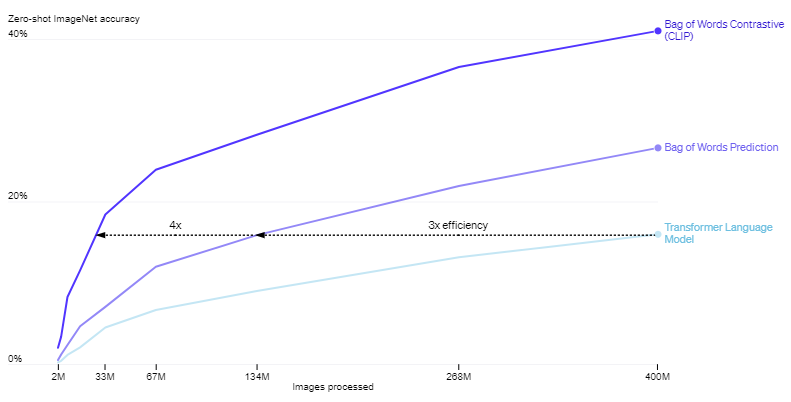
\includegraphics[width=1\textwidth]{clip.png}[~\ref{CLIP efektivita}]
    \caption{CLIP image from OpenAI}
  \end{figure}
\end{frame}



\begin{frame}
  \frametitle{Ďakujem za pozornosť}
  zdroje:
  \begin{itemize}
    \item Ondrej Krajčovič. \textit{Diagram}. 2023. \label{diagram}
    \item Ondrej Krajčovič. \textit{Metadáta}. 2023. \label{metadata}
    \item OpenAI. \textit{CLIP}. 2021. \label{CLIP efektivita}
  \end{itemize}
\end{frame}

\end{document}
